\section{Event Extraction Model}
Once we have automatically labelled a large number of training instances, we can then use the training data to learn an event extractor to
detect the occurrence of events from \emph{unseen} text. In this section, we present a novel neural network based event extractor which
does not rely on explicit trigger information (and hence it eliminates the need for manually labelling triggers when collecting training
data).

%\subsection{Our Task}
Previous event extraction systems mainly rely on explicit trigger identification to detect the occurrence of an event, which is then used
to decide its event type and label its arguments. Because identifying triggers is widely considered as a difficult task, human involvement
is thus required\FIXME{~\cite{}}. In our automatically collected dataset, where human-labeled event triggers are unavailable, we argue that
\textbf{key arguments} can play the same role as explicit event triggers. We thus treat the event extraction as a pipeline of the following
two steps:

\begin{description}
	\item [Event detection]  To identify key arguments in a sentence. If a sentence contains \textbf{all key arguments} of a specific event type, it will be considered to imply an event mention of this specified type.
	\item [Argument detection] To identify other non-key arguments for each event in the sentence.
\end{description}
%
Take S1 as an example, in event detection, \emph{Remedy Corp}, \emph{BMC Software}, and \emph{2004} could be identified as
\texttt{company\_acquired}, \texttt{acquiring\_company}, and \texttt{date}, respectively, indicating that S1 may mention a
\texttt{business.acquisition} event. During argument detection, \emph{Service Management Business Unit} should be identified as
\texttt{divisions\_formed}, which, together with the detected key arguments, form a full mention for a \texttt{business.acquisition} event.

\subsection{Event Detection \label{evede}}
%Before presenting our model,
%Our event detector is an BLSTM-CRF model with ILP-based inference.
%We first present our solution for multi-words arguments, and then introduce each component in our model.
%BLSTM-CRF-ILP$_{multi}$ model, from bottom to top.

%\paragraph{Tagging scheme}
There are 68\%  of  arguments in our dataset consist of more than one word. We thus formulate each subtask in a sequence labeling paradigm
rather than word-level classifications. Each word in the given sentence is tagged with the widely used begin-inside-outside (\texttt{BIO})
scheme\FIXME{\cite{}}, where each token is labeled as \texttt{B-role} if it is the beginning of an event argument with its corresponding
role \texttt{role}, or \texttt{I-role} if it is inside an argument, or \texttt{O} otherwise.


Figure~\ref{fig:model} provides an overview of our event detection model. Our event detection model has two key components, a bidirectional
LSTM (BLSTM) model with a conditional random field (CRF) layer and a Integer Linear Programming (ILP) based post inference. The input to
our model is the raw text. The embedding layer maps the input text to a vector of real values, where each token of the text is mapped to an
integer value. The BLSTM and CRF layers find the optimal label sequence which will then be post-processed by the ILP-based layer.

\begin{figure}
  \centering
  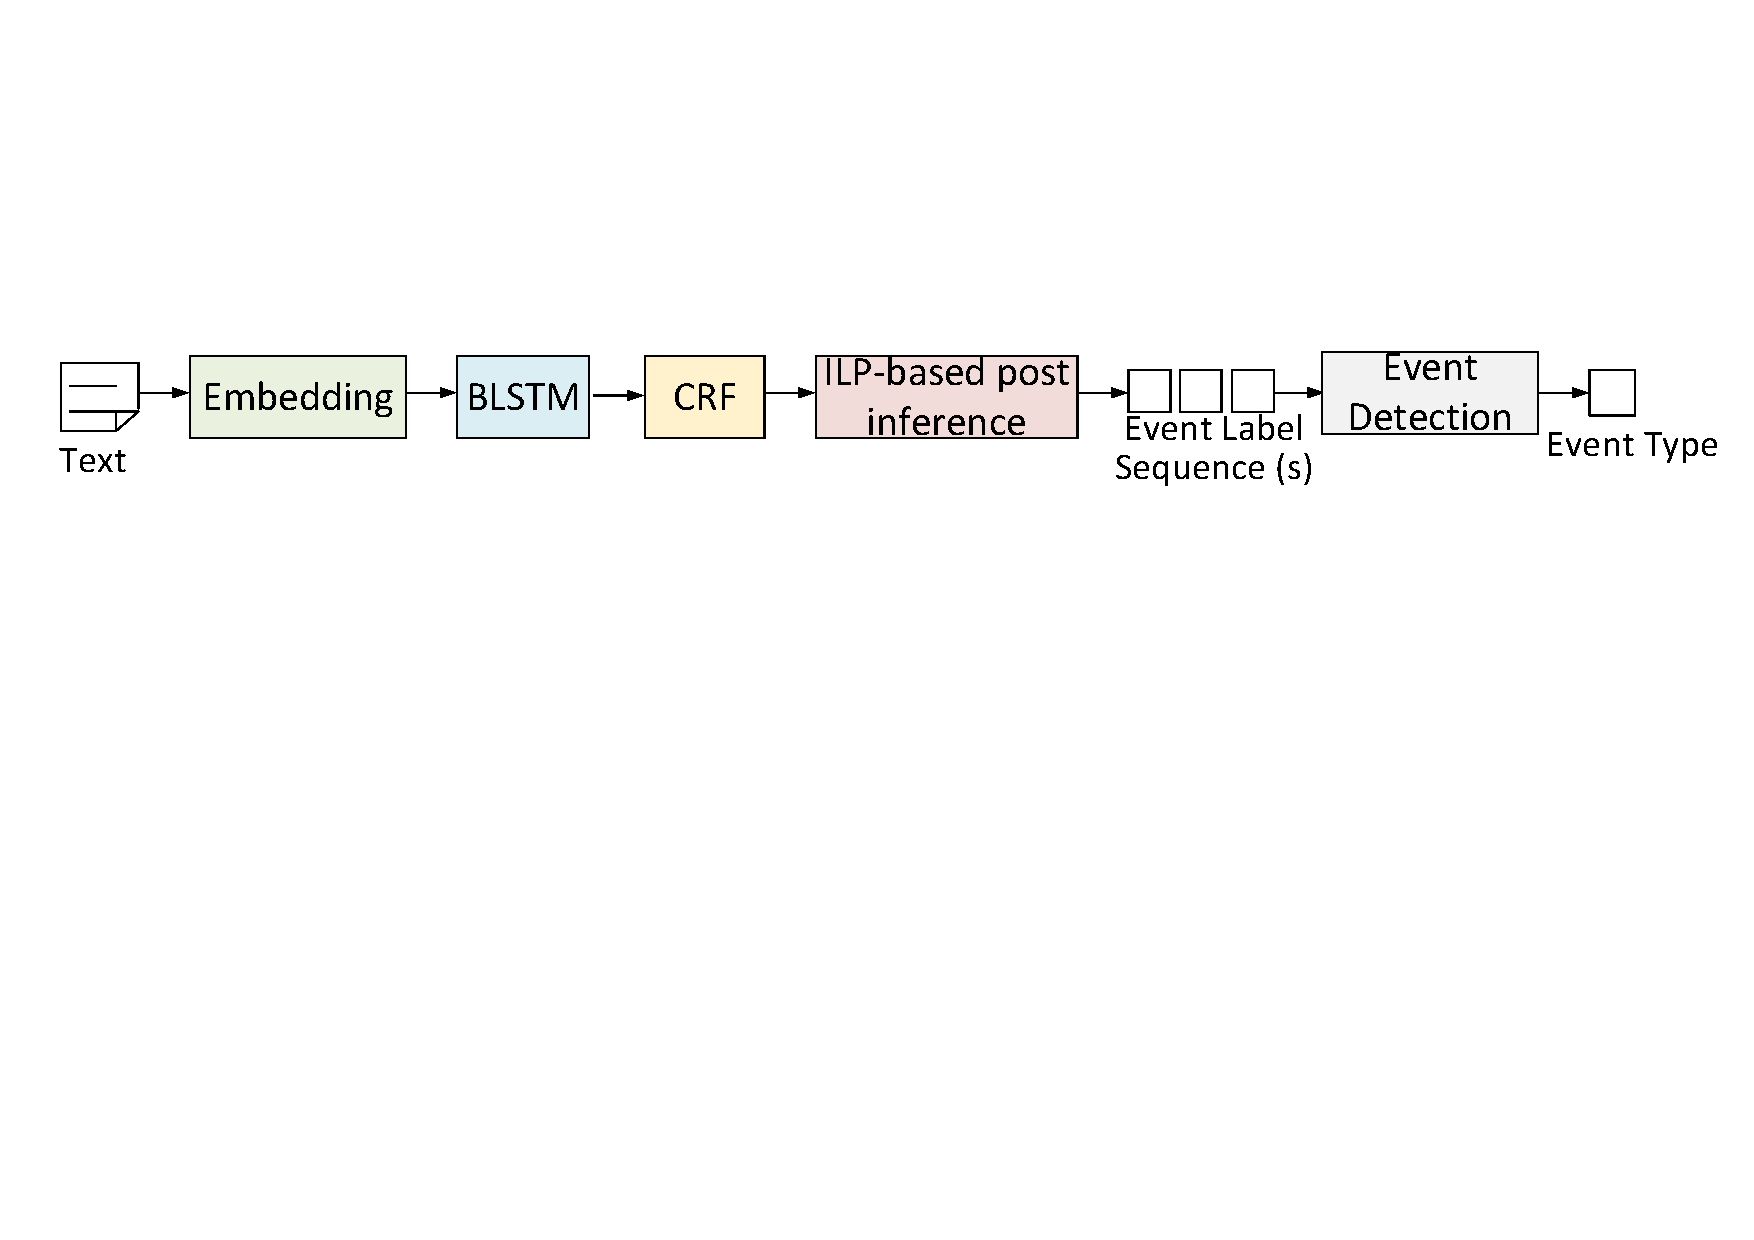
\includegraphics[width=0.5\textwidth]{figs/model.pdf}
  \caption{Our event detection model.}\label{fig:model}
\end{figure}

\paragraph{BLSTM}
The Long Short-Term Memory Network (LSTM)~\cite{hochreiter1997long} is a natural fit for sequence labeling, which maintains a memory based
on historical contextual information. Formally, given a sentence $\bm{w} = \{w_1, w_2, \dots, w_n\}$ of length $n$, we use $\textbf{x}_t$
to represent feature vector, e.g., word embeddings, corresponding to the $t$-th word $w_t$. At each time $t$, a forward LSTM layer takes
$\textbf{x}_t$ as input and computes the output vector $\overrightarrow{\textbf{h}}_t$ of the past context, while a backward LSTM layer
reads the same sentence in reverse and outputs $\overleftarrow{\textbf{h}}_t$ given the future context. We concatenate these two vectors to
form the output vector of a BLSTM, which is fed into a softmax layer to estimate a probability distribution over all possible labels.

\paragraph{CRF}
A straightforward way to find the label sequence for given sentence is to choose the
best label for each word individually according to the BLSTM output.
%with maximum probability by LSTM as the prediction for each word.
However, this greedy strategy ignores the dependencies between labels, thus cannot guarantee the best sequence.  %this independent labeling strategy
%is limited especially when there are strong dependencies and constraints between labels.
%To model the correlations between labels,
Therefore, we introduce a CRF layer over the BLSTM output, which is shown to be effective in various sequence labeling tasks~\cite{collobert2011natural,huang2015bidirectional}. %, such as POS tagging and NER .

We consider $\textbf{P}$ to be a matrix of confidence scores output by BLSTM, and the element $\textbf{P}_{i,j}$ of the matrix denotes the probability of the label $j$ for the $i$-th word in a sentence. The CRF layer takes a transition matrix $\textbf{A}$ as parameter, where $\textbf{A}_{i,j}$ represents the score of a transition from label $i$ to label $j$. The score of a sentence $\bm{w}$ along with a path of labels $\bm{y} = \{y_1, y_2, \ldots, y_n\}$ is measured by the sum of BLSTM outputs and transition scores:
\begin{equation}
	score(\bm{w}, \bm{y}) = \sum\limits_{i=0}^n\textbf{P}_{i, y_i} + \sum\limits_{i=1}^n\textbf{A}_{y_i, y_{i+1}},
\end{equation}
During test, given a sentence $\bm{w}$, we adopt the Viterbi algorithm~\cite{rabiner1989tutorial} to find the optimal label sequence with the maximum score among all possible label sequences.

\paragraph{ILP-based Post Inference}
Essentially, event detection is a structure prediction problem. However, the output sequences of BLSTM-CRF do not necessarily satisfy the
structural constraints. For instance, regardless of how many key arguments are correctly identified by BLSTM-CRF, if there is one key
argument missing, this detection should be considered as failed.

We thus propose to apply ILP to further globally optimize the BLSTM-CRF output  to produce the best label sequence. Formally, let
$\mathcal{L}$ be the set of possible argument labels. For each word $w_i$ in the sentence $\bm{w}$ and a pair of labels $ \langle l, l'
\rangle \in \mathcal{L} \times \mathcal{L}$, we create a binary variable ${v_{i,l,l'} \in \{0, 1\}}$, denoting whether or not the $i$-th
word $w_i$ is tagged as label $l$ and its following word $w_{i+1}$ is tagged as label $l'$ at the same time. The objective of ILP is to
maximize the overall score of the variables as:
\begin{displaymath}
	\sum\nolimits_{i, l, l'}v_{i,l,l'} * (\textbf{P}_{i,l}+\textbf{A}_{l,l'}) .
\end{displaymath}
where we consider the following four constraints:

\textbf{C1}: Each word should be and only be annotated with one label, i.e.:
\begin{equation}
	\sum\nolimits_{l,l'}v_{i,l,l'}=1
\end{equation}

\textbf{C2}: If the value of $v_{i,l,l'}$ is $1$, then there has to be a label $l^*$ that will make $v_{i+1,l',l^*}$ equal to $1$, i.e.:
\begin{equation}
	v_{i,l,l'} = \sum\nolimits_{l^*}v_{i+1,l',l^*}
\end{equation}

\textbf{C3}: If the current label is \texttt{I-arg}, then its previous label must be \texttt{B-arg} or \texttt{I-arg}, i.e.:
\begin{equation}
	v_{i,\texttt{I-arg},l'} = v_{i-1,\texttt{B-arg},\texttt{I-arg}} + v_{i-1, \texttt{I-arg}, \texttt{I-arg}}
\end{equation}

\textbf{C4}: For a specific event type, all its key arguments should co-occur in the sentence, or none of them appears in the resulting sequence. For any pair of key arguments $arg_1$ and $arg_2$ with respect to the same event type, the variables related to them are subject to:
\begin{equation}
	\sum\nolimits_{i,l'}{v_{i,\texttt{B-arg}_1,l'}} \leq n * \sum\nolimits_{j,l^*}{v_{j,\texttt{B-arg}_2,l^*}}
\end{equation}
where $n$ is the length of the sentence.

\paragraph{Multi-typed Events}
There are scenarios where one event is associated with multiple types, but all current event extractors only map a sentence to one event.
\FIXME{zw: we need an example here.} One of the advantages of our approach is that it can be easily extended to support multi-typed events.
To do so, we allow our ILP solver to output multiple optimal sequences. Specifically, after our model outputs the best sequence $\bm{s}^t$
at time $t$, we remove the previously best solutions
 $\{\bm{s}^1, \ldots, \bm{s}^{t}\}$ from the solution space, and re-run our solver to obtain the next optimal sequences $\bm{s}^{t+1}$.
We repeat the optimization procedure until the difference between the scores of $\bm{s}^1$ and $\bm{s}^T$ is greater
than a threshold $\lambda$, and consider all solutions $\{\bm{s}^1, \bm{s}^2, \ldots, \bm{s}^{T-1}\}$ as the optimal label sequences.
We use Gurobi~\cite{gurobi} as our ILP solver and set $\lambda=0.05 \times n$, which averagely produce~1.07 optimal sequences for each sentence.

\subsection{Argument Detection}
After event detection, a sentence will be classified into different event types, and labeled with its corresponding key arguments.
%The next step is argument detection, which
Next, we will identify the remaining non-key arguments in the sentence.

We adopt the same BLSTM-CRF architecture (in Sec~\ref{evede}) for argument detection, where we encode the event label (output of event detection) of each word into a key-argument feature vector through a look-up table, and concatenate it with the original word embedding as the input to the new BLSTM-CRF. Note that we do not need post inference here.
